  \subsection{Análisis de una forma de onda cuadrada}
    Se propone realizar el análisis en frecuencia de una señal de forma cuadrada, recordando que
    su espectro posee, de forma ideal, infinitos armónicos impares. Lo primero que se realiza es 
    la calibración de las puntas del osciloscopio.

    Luego, se conecta el generador al osciloscopio configurado con una \textbf{onda cuadrada} de
    frecuencia $\mathbf{f=1~kHz}$, y amplitud arbitraria. El menú del canal 1 se configura de la
    siguiente manera: \textbf{Acoplamiento CC}, \textbf{Sin límite de ancho de banda},
    \textbf{Sonda x10} y \textbf{No invertido}. Luego, para poder observar el espectro se
    se configura el menú matemático como sigue: \textbf{FFT}, \textbf{CH1}, \textbf{Rectangular},
    y \textbf{Zoom x1}. La Figura~\ref{fig:SeñalCuad1k} muestra esta señal en tiempo y frecuencia.

    \begin{figure}[H]
      \centering
      \begin{subfigure}[H]{0.42\textwidth}
        \frame{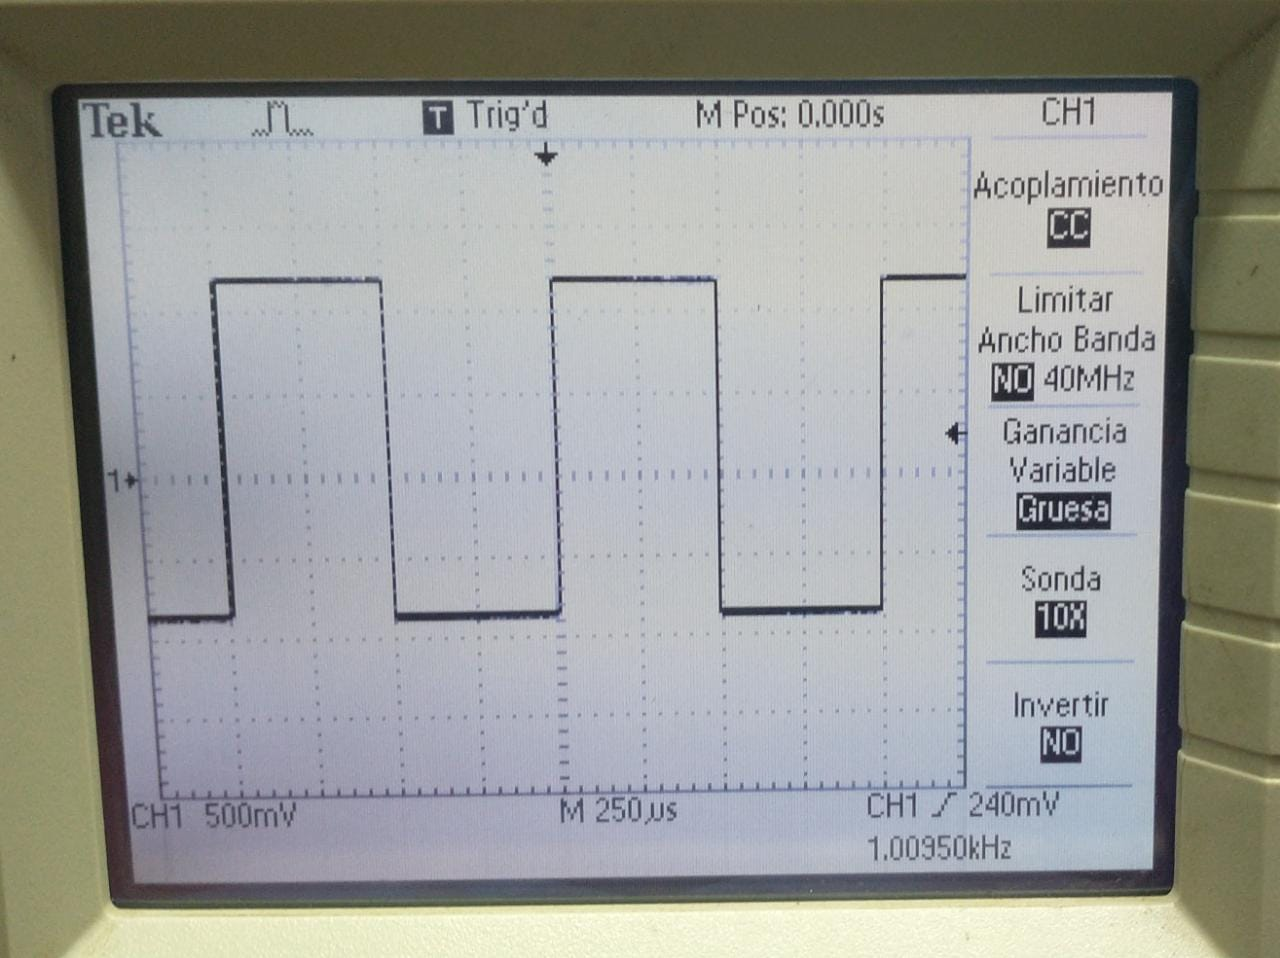
\includegraphics[width=\textwidth]{Imagenes/ActividadPractica/1AnalisisDeUnaSeñalCuadrada/Exp1_SeñalCuadrada1k_tiempo.jpeg}}
        \caption{En tiempo.}
      \end{subfigure}
      \hfill 
      \begin{subfigure}[H]{0.44\textwidth}
        \frame{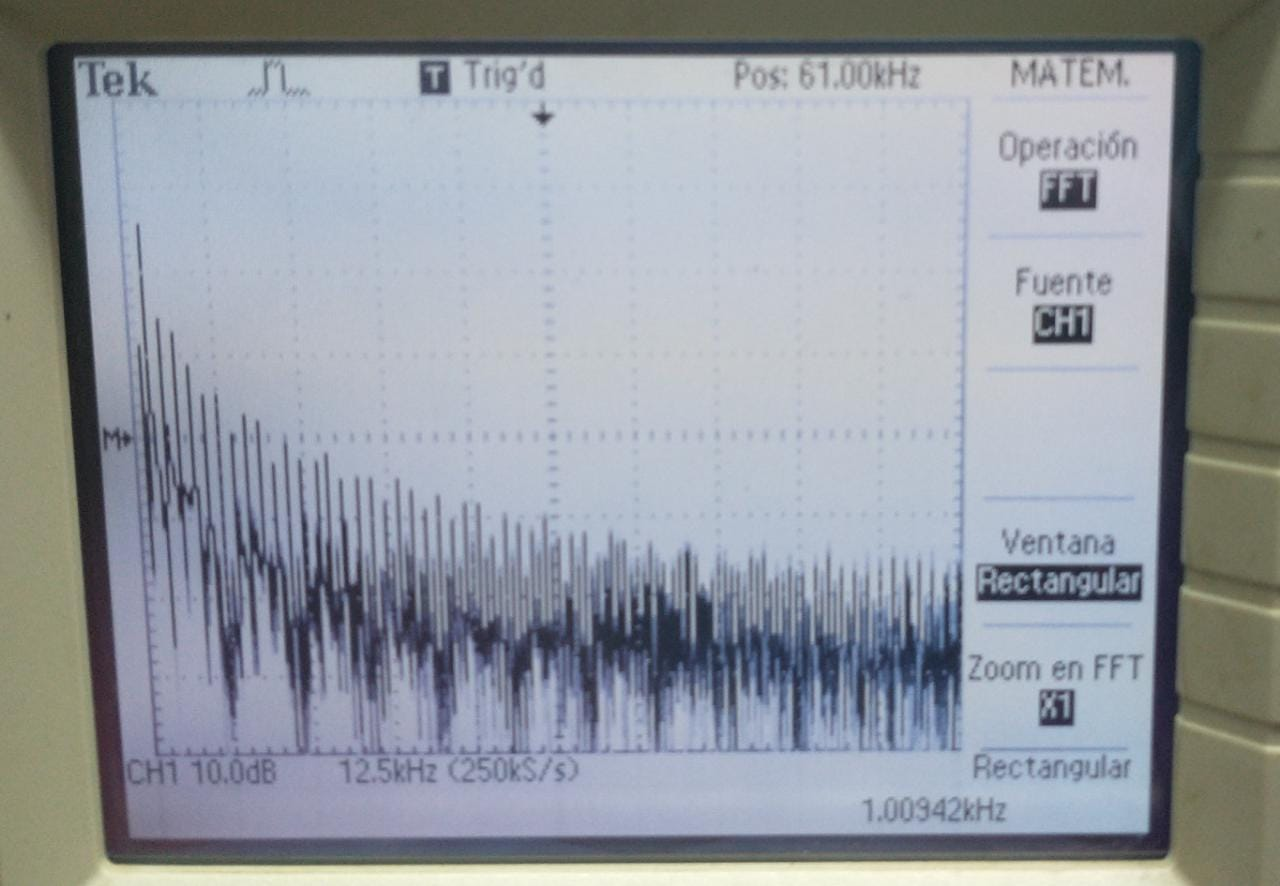
\includegraphics[width=\textwidth]{Imagenes/ActividadPractica/1AnalisisDeUnaSeñalCuadrada/Exp1_SeñalCuadrada1k_frec.jpeg}}
        \caption{En frecuencia.}
      \end{subfigure}

      \caption{Señal cuadrada de $1~kHz$.}
      \label{fig:SeñalCuad1k}
    \end{figure}

    A continuación, se procede a analizar los tipos de \textbf{adquisión} y \textbf{ventanas} con la misma señal
    previamente configurada. Para ello, se elige la opción \textbf{Zoom x10}. En la Figura~\ref{fig:SeñalCuadModoNormal}
    se muestran las distintas ventanas para el modo de adquisición \textbf{normal}.

    \begin{figure}[H]
      \centering
      \begin{subfigure}[H]{0.40\textwidth}
        \frame{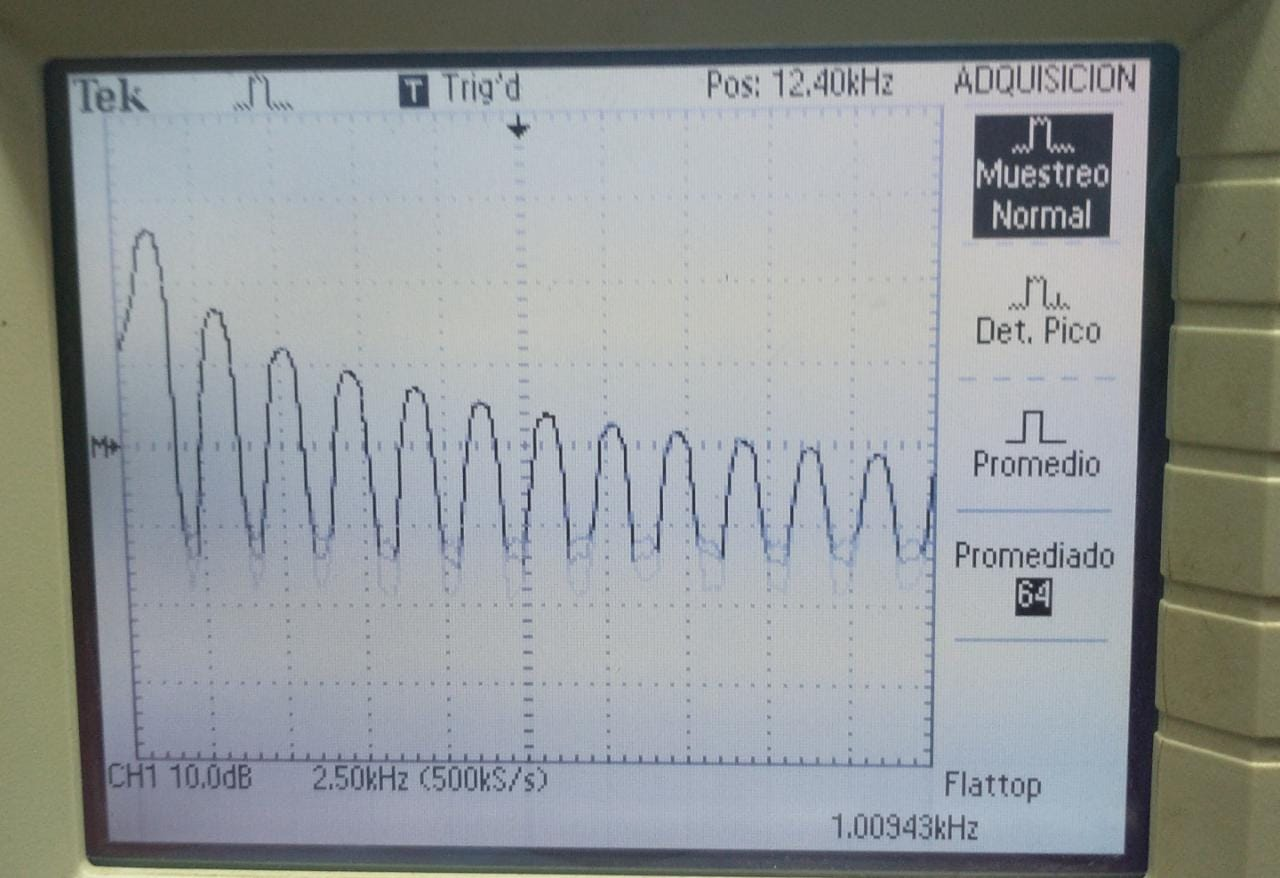
\includegraphics[width=\textwidth]{Imagenes/ActividadPractica/1AnalisisDeUnaSeñalCuadrada/Exp1_SeñalCuadrada_Normal_Flattop.jpeg}}
        \caption{Con ventana Flattop.}
      \end{subfigure}
      \hfill 
      \begin{subfigure}[H]{0.39\textwidth}
        \frame{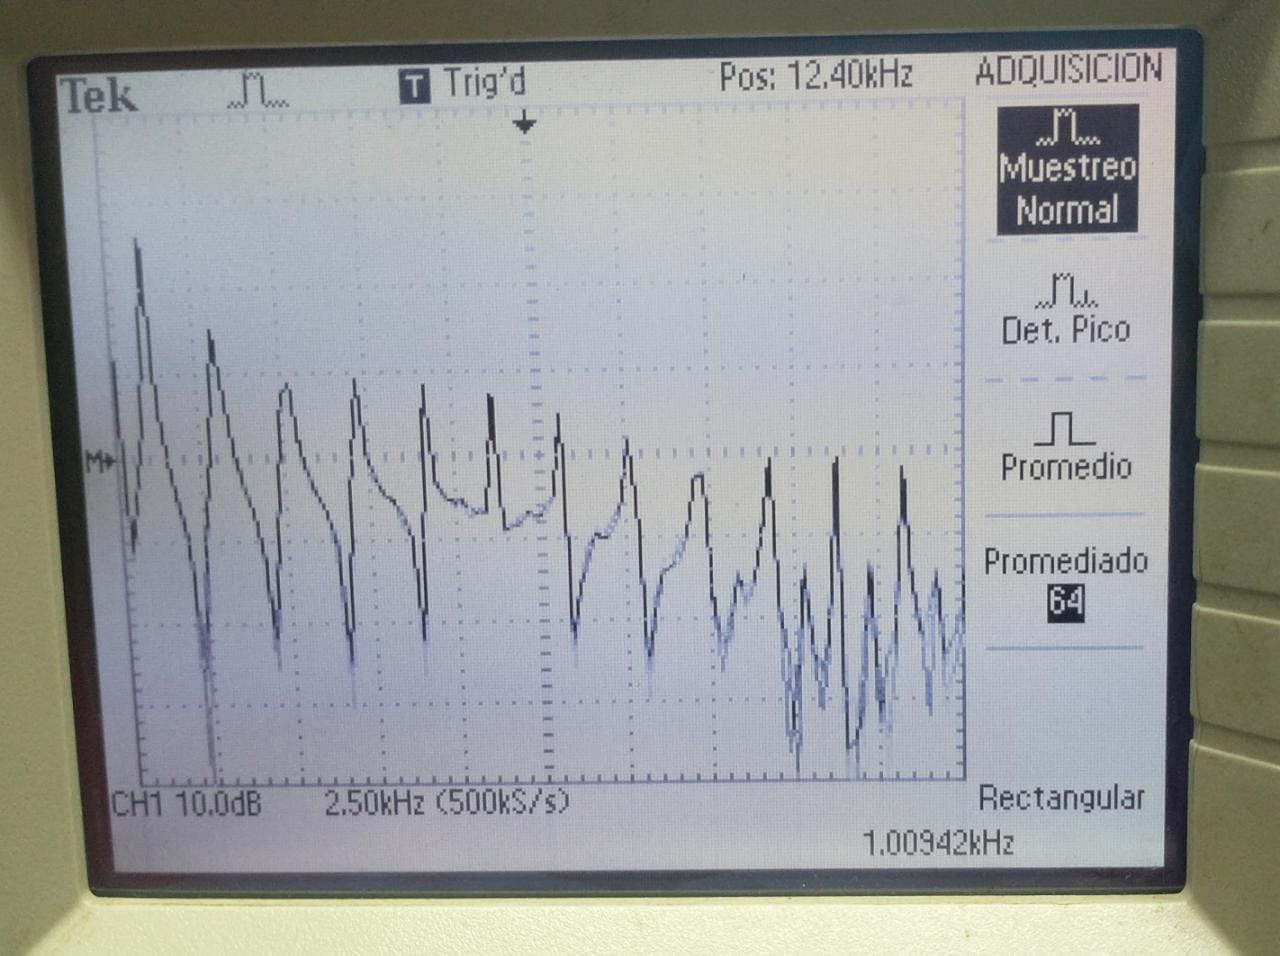
\includegraphics[width=\textwidth]{Imagenes/ActividadPractica/1AnalisisDeUnaSeñalCuadrada/Exp1_SeñalCuadrada_Normal_Rectangular.jpeg}}
        \caption{Con ventana Rectangular.}
      \end{subfigure}
      \hfill 
      \begin{subfigure}[H]{0.40\textwidth}
        \frame{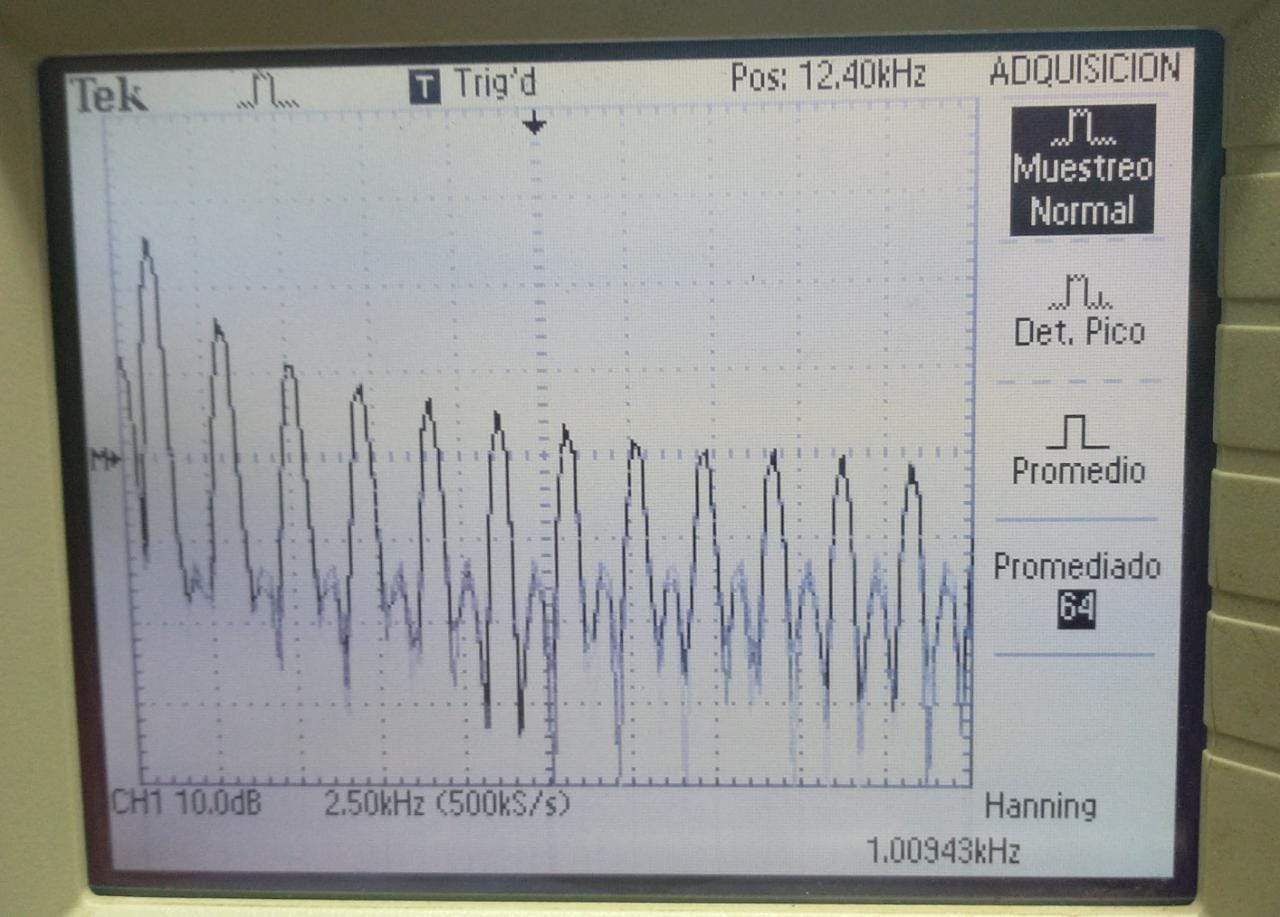
\includegraphics[width=\textwidth]{Imagenes/ActividadPractica/1AnalisisDeUnaSeñalCuadrada/Exp1_SeñalCuadrada_Normal_Hanning.jpeg}}
        \caption{Con ventana de Hanning.}
      \end{subfigure}

      \caption{Señal cuadrada de $1~kHz$ con modo de adquisición normal..}
      \label{fig:SeñalCuadModoNormal}
    \end{figure}

    Ahora, se selecciona el modo de adquisicón de \textbf{detección de picos} y se varían los tipos de ventanas.
    Esto se encuentra en la Figura~\ref{fig:SeñalCuadModoDetecPicos}.
    \begin{figure}[H]
      \centering
      \begin{subfigure}[H]{0.40\textwidth}
        \frame{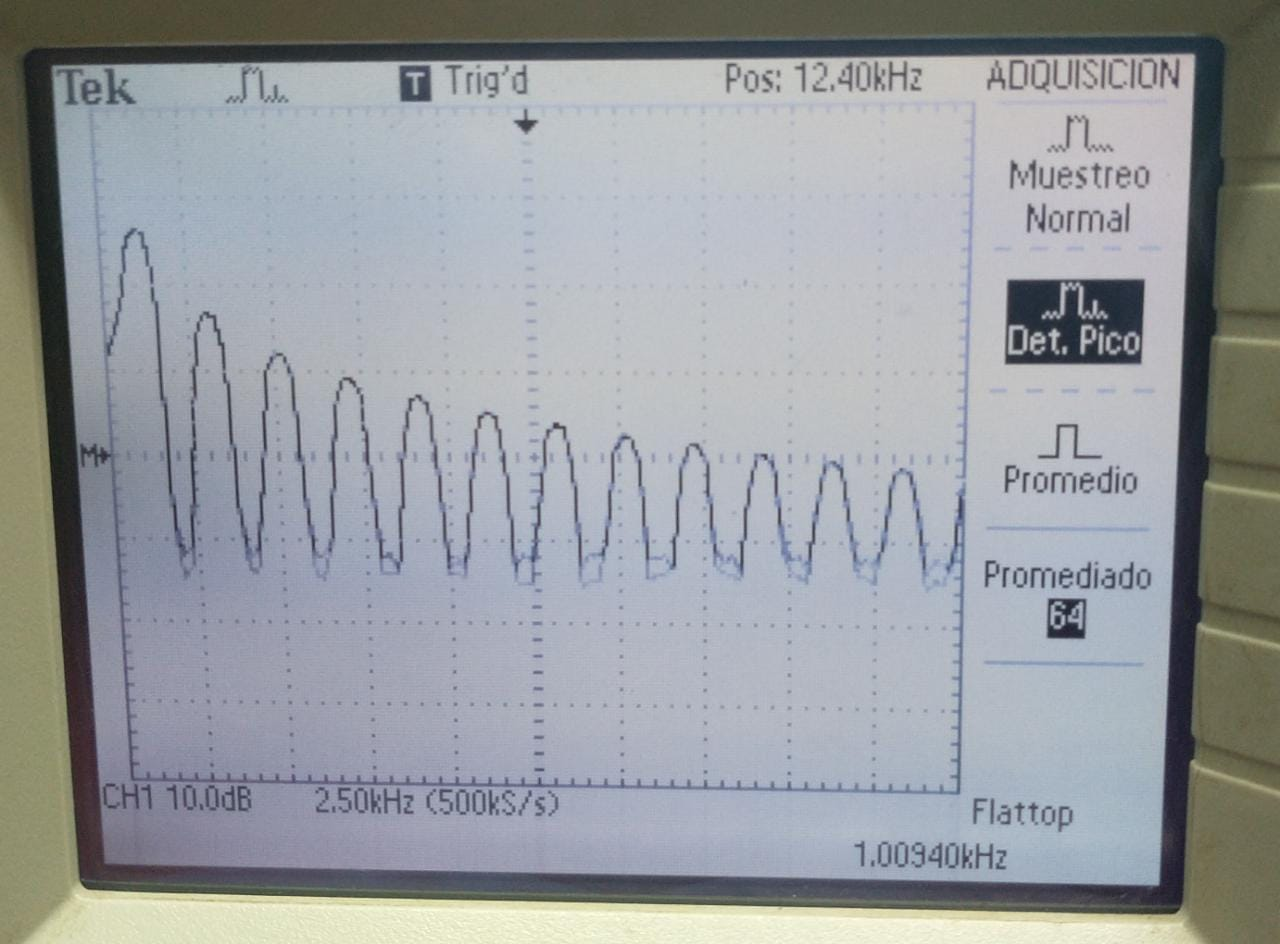
\includegraphics[width=\textwidth]{Imagenes/ActividadPractica/1AnalisisDeUnaSeñalCuadrada/Exp1_SeñalCuadrada_DecPicos_Flattop.jpeg}}
        \caption{Con ventana Flattop.}
      \end{subfigure}
      \hfill 
      \begin{subfigure}[H]{0.40\textwidth}
        \frame{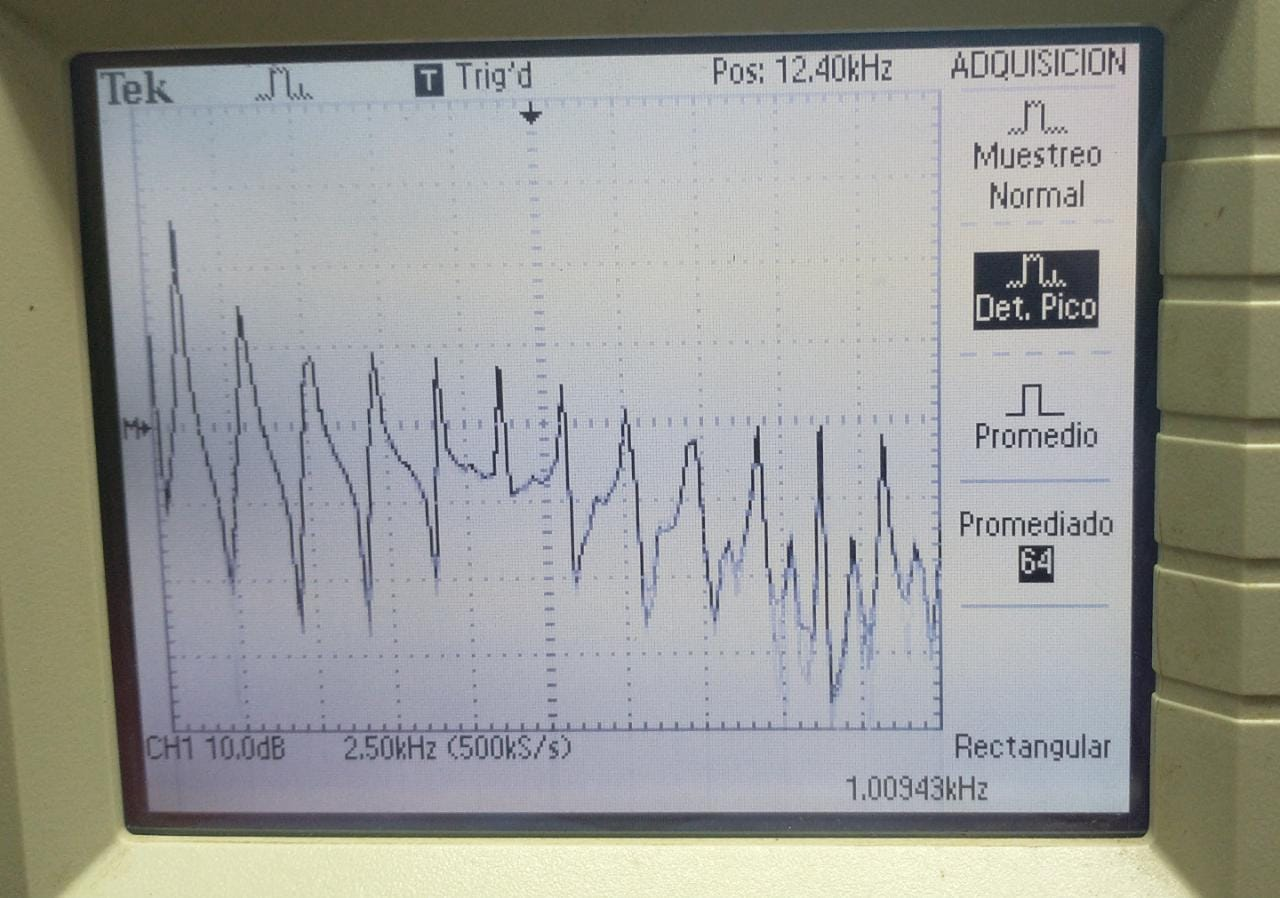
\includegraphics[width=\textwidth]{Imagenes/ActividadPractica/1AnalisisDeUnaSeñalCuadrada/Exp1_SeñalCuadrada_DecPicos_Rectangular.jpeg}}
        \caption{Con ventana Rectangular.}
      \end{subfigure}
      \hfill 
      \begin{subfigure}[H]{0.40\textwidth}
        \frame{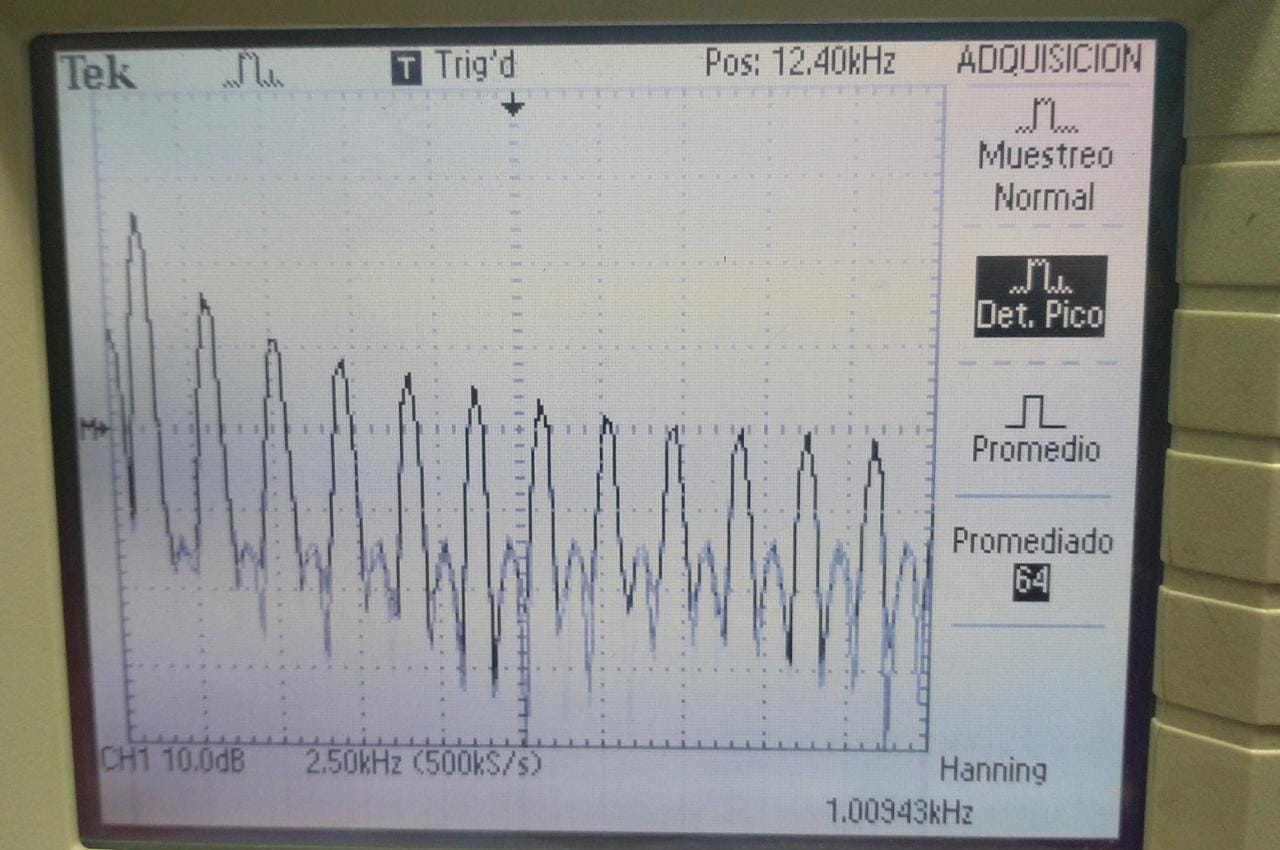
\includegraphics[width=\textwidth]{Imagenes/ActividadPractica/1AnalisisDeUnaSeñalCuadrada/Exp1_SeñalCuadrada_DecPicos_Hanning.jpeg}}
        \caption{Con ventana de Hanning.}
      \end{subfigure}

      \caption{Señal cuadrada de $1~kHz$ con modo de adquisición de detección de picos.}
      \label{fig:SeñalCuadModoDetecPicos}
    \end{figure}

    Finalmente, se pone a prueba el modo de adquisición \textbf{promedios}, para el cual se eligen
    \textbf{64 cuentas}. Esto se encuentra en la Figura~\ref{fig:SeñalCuadModoPromedio}.

    \begin{figure}[H]
      \centering
      \begin{subfigure}[H]{0.40\textwidth}
        \frame{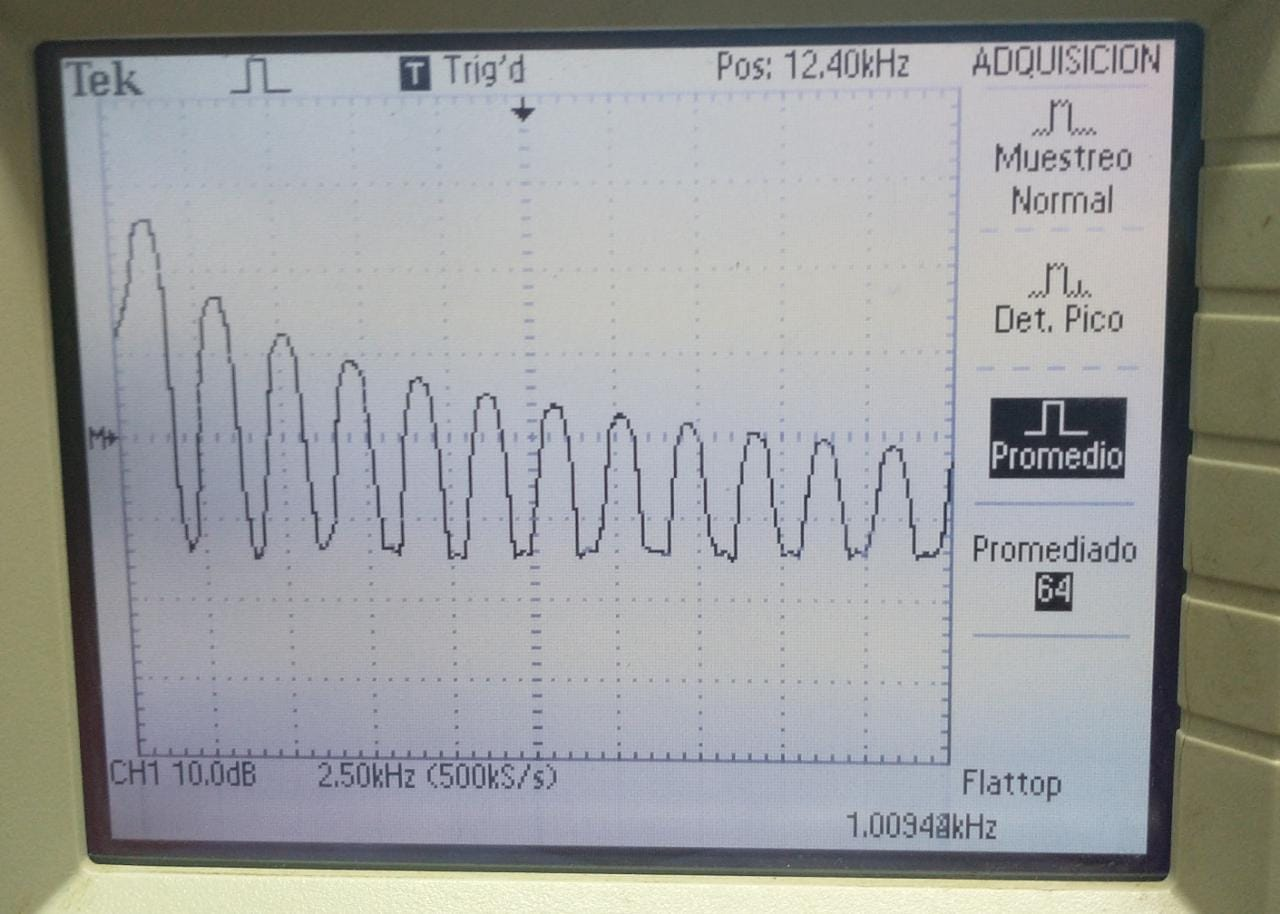
\includegraphics[width=\textwidth]{Imagenes/ActividadPractica/1AnalisisDeUnaSeñalCuadrada/Exp1_SeñalCuadrada_Promedio_Flattop.jpeg}}
        \caption{Con ventana Flattop.}
      \end{subfigure}
      \hfill 
      \begin{subfigure}[H]{0.40\textwidth}
        \frame{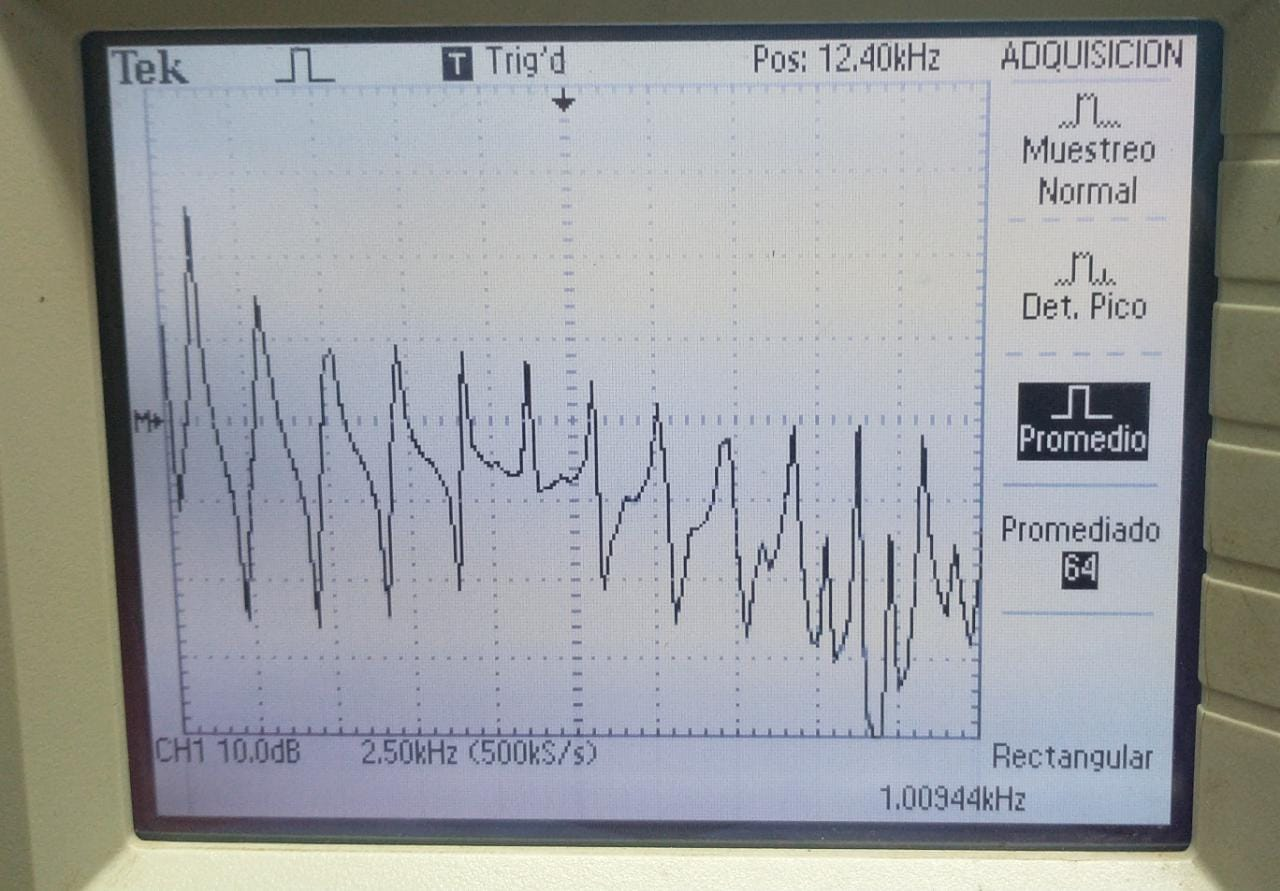
\includegraphics[width=\textwidth]{Imagenes/ActividadPractica/1AnalisisDeUnaSeñalCuadrada/Exp1_SeñalCuadrada_Promedio_Rectangular.jpeg}}
        \caption{Con ventana Rectangular.}
      \end{subfigure}
      \hfill 
      \begin{subfigure}[H]{0.40\textwidth}
        \frame{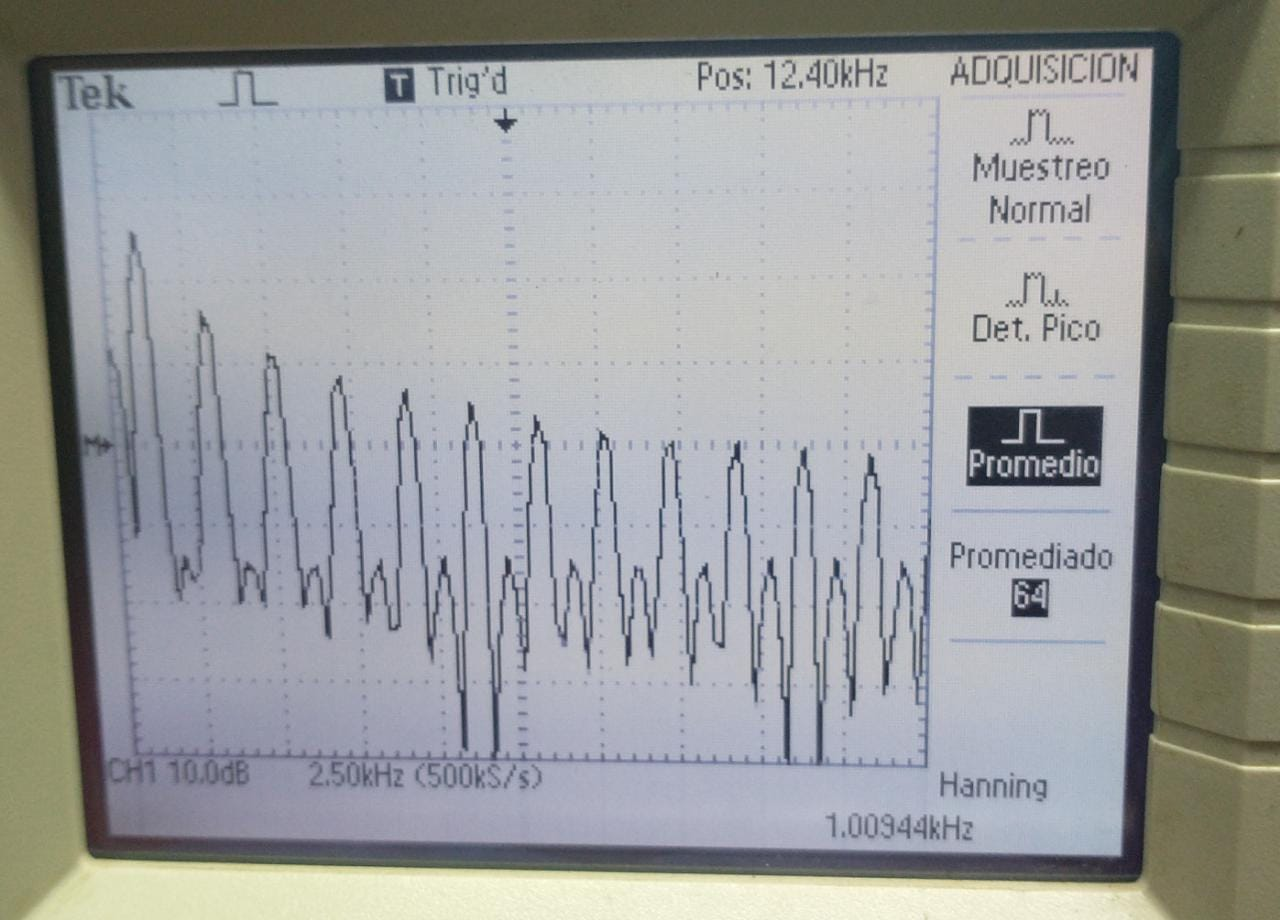
\includegraphics[width=\textwidth]{Imagenes/ActividadPractica/1AnalisisDeUnaSeñalCuadrada/Exp1_SeñalCuadrada_Promedio_Hanning.jpeg}}
        \caption{Con ventana de Hanning.}
      \end{subfigure}

      \caption{Señal cuadrada de $1~kHz$ con modo de adquisición de promedios.}
      \label{fig:SeñalCuadModoPromedio}
    \end{figure}

    
    \subsubsection{Medición de frecuencia}

      \begin{table}[H]
        \centering
      \begin{tabular}{cccccccc} \hline \hline
        \textbf{Comp. Espectral}  &  \textbf{1}  &  \textbf{2}  & \textbf{3}  & \textbf{4} & \textbf{5}  & \textbf{6}  &  \textbf{7}\\ \hline
        \textbf{Frec. [kHz]}   &   $1,0$   &    $3,0$   &   $5,1$  &  $7,1$  &  $9,1$  &  $11,0$  &  $13,0$\\ \hline \hline
        \end{tabular}
        \caption{Frecuencias de las primeras 7 componentes espectrales.}
        \label{tab:ComponentesEspectrExp1}
      \end{table}


    \subsubsection{Medición de amplitud}


      \begin{table}[H]
        \centering
      \begin{tabular}{cccccccc} \hline \hline
        \textbf{Comp. Espectral}  &  \textbf{1}  &  \textbf{2}  & \textbf{3}  & \textbf{4} & \textbf{5}  & \textbf{6}  &  \textbf{7}\\ \hline
        \textbf{Tensión}   &   $V_1$   &    $V_2$   &   $V_3$  &  $V_4$  &  $V_5$  &  $V_6$  &  $V_7$\\ \hline \hline
        \textbf{[dBv]}   &   $-790m$   &    $-10,2$   &   $-14,6$  &  $-17,8$  &  $-20$  &  $-21,4$  &  $-23,3$\\ \hline
        \textbf{[V]}     &  $0,91$     &    $0,31$    & $0,19$     &  $0,13$   &  $0,1$  &  $0,09$   &  $0,07$ \\ \hline
        $\mathbf{[V^2]}$ &  $0,83$     &    $0,09$    & $0,03$     &  $0,02$   &  $0,01$ &  $0,007$  &  $0,005$ \\ \hline \hline
        \end{tabular}
        \caption{Amplitudes de las primeras 7 componentes espectrales.}
        \label{tab:AmplitudEspectrExp1}
      \end{table}

    \pagebreak
